\documentclass[11pt,oneside]{book}
\usepackage[backend=biber,natbib=true,style=alphabetic,maxbibnames=10]{biblatex}
\addbibresource{/home/nqbh/reference/bib.bib}
\usepackage[utf8]{vietnam}
\usepackage{tocloft}
\renewcommand{\cftsecleader}{\cftdotfill{\cftdotsep}}
\usepackage[colorlinks=true,linkcolor=blue,urlcolor=red,citecolor=magenta]{hyperref}
\usepackage{amsmath,amssymb,amsthm,chemfig,float,graphicx,mathtools,multicol,soul}
\usepackage[version=4]{mhchem}
\allowdisplaybreaks
\newtheorem{assumption}{Assumption}
\newtheorem{baitoan}{Bài toán}
\newtheorem{cauhoi}{Câu hỏi}
\newtheorem{conjecture}{Conjecture}
\newtheorem{corollary}{Corollary}
\newtheorem{dangtoan}{Dạng toán}
\newtheorem{definition}{Definition}
\newtheorem{dinhly}{Định lý}
\newtheorem{dinhnghia}{Định nghĩa}
\newtheorem{example}{Example}
\newtheorem{goal}{Goal}
\newtheorem{ghichu}{Ghi chú}
\newtheorem{hequa}{Hệ quả}
\newtheorem{hypothesis}{Hypothesis}
\newtheorem{lemma}{Lemma}
\newtheorem{luuy}{Lưu ý}
\newtheorem{muctieu}{Mục tiêu}
\newtheorem{nhanxet}{Nhận xét}
\newtheorem{notation}{Notation}
\newtheorem{note}{Note}
\newtheorem{principle}{Principle}
\newtheorem{problem}{Problem}
\newtheorem{proposition}{Proposition}
\newtheorem{question}{Question}
\newtheorem{remark}{Remark}
\newtheorem{theorem}{Theorem}
\newtheorem{vidu}{Ví dụ}
\usepackage[margin=2cm,footskip=1cm]{geometry}
\def\labelitemii{$\circ$}
\DeclareRobustCommand{\divby}{%
	\mathrel{\vbox{\baselineskip.65ex\lineskiplimit0pt\hbox{.}\hbox{.}\hbox{.}}}%
}

\title{Some Topics in Elementary STEM \textit{\&} Beyond:\\A Personal, Psychological, \textit{\&} Philosophical Perspective\\\vspace{1cm}
	\textsf{\Large Vài Vấn Đề Trong STEM Sơ Cấp \& Xa Hơn Thế:\\1 Góc Nhìn Cá Nhân, Tâm Lý Học, \& Triết Học.}}
\author{Nguyễn Quản Bá Hồng\footnote{A Scientist- \& Creative Artist Wannabe, Ben Tre City, Vietnam\\e-mail: \texttt{nguyenquanbahong@gmail.com}; website: \url{https://nqbh.github.io}.}}
\date{\textsf{Version: \today}}

\begin{document}
\maketitle
\begin{quotation}
	\textit{``In this world, is the destiny of mankind controlled by some transcendental entity or law? Is it like the hand of God hovering above? At least it is true that man has no control, even over his own will. Man takes up the sword in order to shield the small wound in his heart sustained in a far-off time beyond remembrance. Man wields the sword so that he may die smiling in some far-off time beyond perception.''} -- \textsc{Kentaro Miura}, \textit{Berserk}, Vol. 1
	\begin{figure}[H]
		\centering
		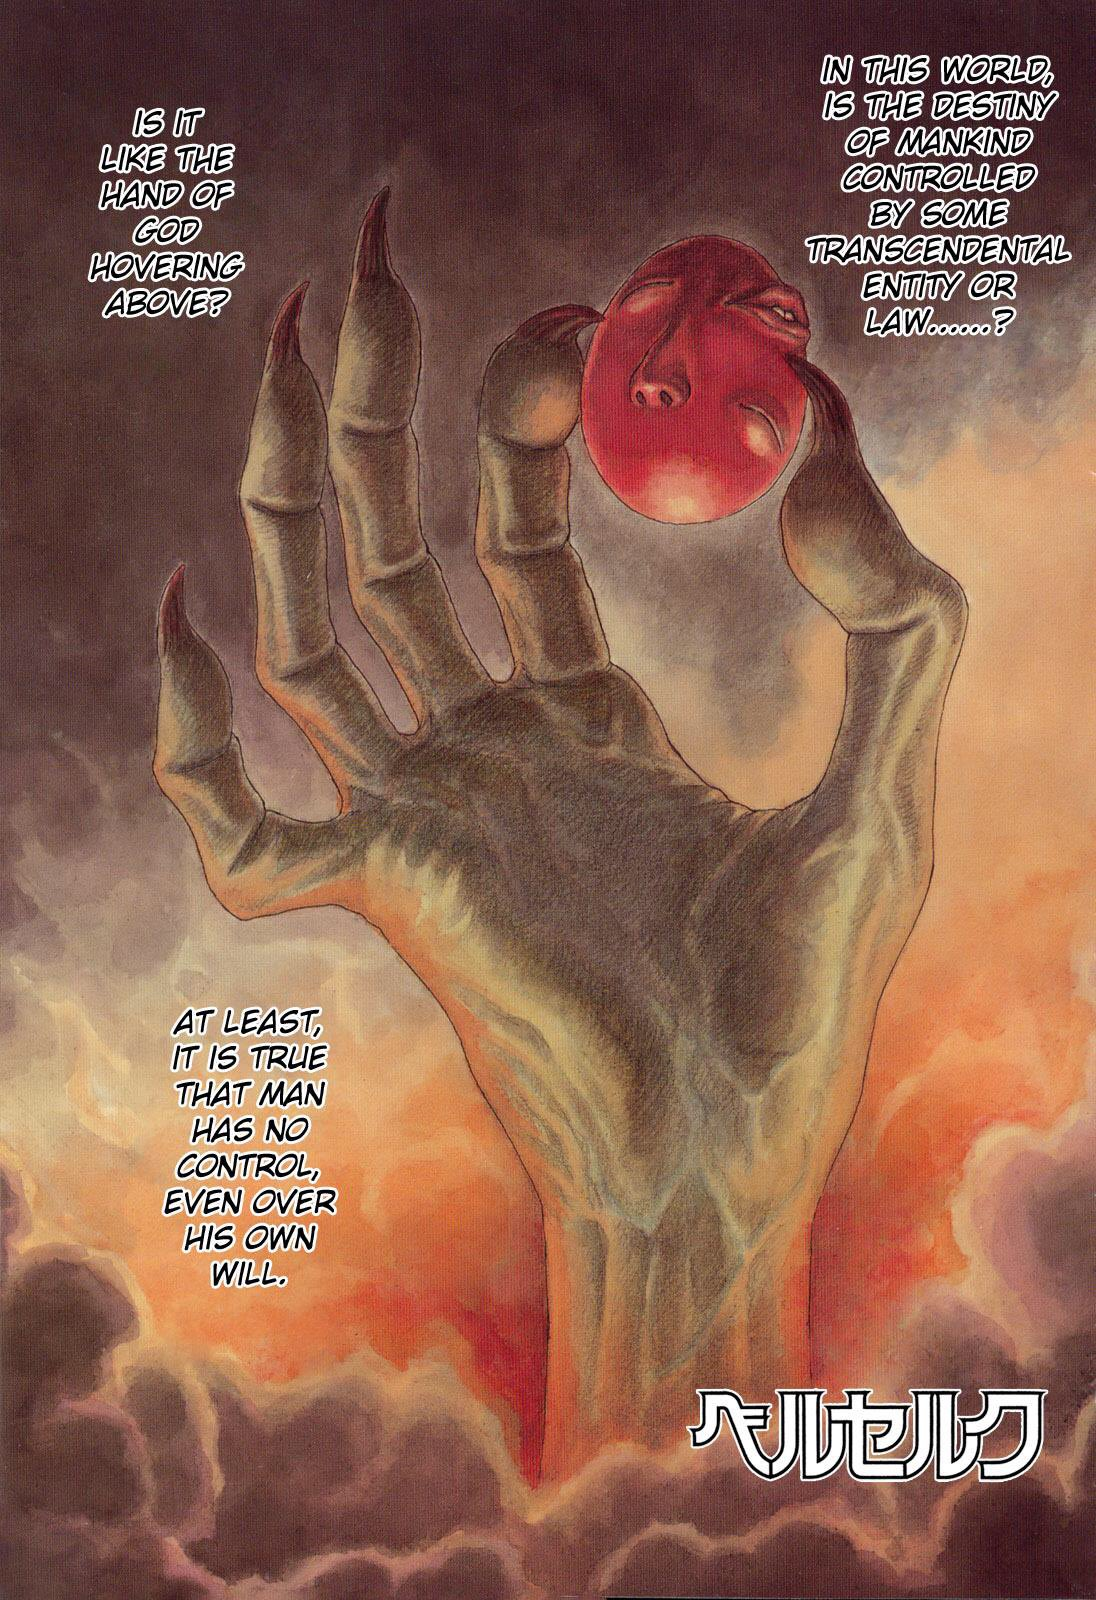
\includegraphics[scale=.15]{Berserk_behelit_color}
		\caption{Berserk, The Hand of God \textit{\&} Behelit.}
	\end{figure}	
	\textit{``Providence may guide a man to meet 1 specific person, even if such guidance eventually leads him to darkness. Man simply cannot forsake the beauty of his own chosen path. When will man learn a way to control his soul?''} – \textsc{Kentaro Miura}, \textit{Berserk}
\end{quotation}
\hrule
\begin{multicols}{2}
	\textit{``What are you doing actually?''} ``I am writing a book.'' \textit{``About what?''} ``I don't know yet.'' \textit{``Huh? You want to write a book but you don't know specifically what to write yet? How can that be?''} ``Everything starts with a sheer will to write, I suppose.'' \textit{``What a joke!''} ``Yeah, let my innocent Infinite Jest \footnote{\textit{Infinite Jest} is the name of a book written by \textsc{David Foster Wallace}, a genius, suicide in ??.} begin.''
	\columnbreak
	
	\textit{``Thực sự là mày đang làm gì vậy?''} ``Tui đang viết 1 cuốn sách.'' \textit{``Về cái gì?''} ``Tui cũng chưa biết nữa.'' \textit{``Hả, mày muốn viết 1 cuốn sách nhưng mày chưa biết viết cụ thể về cái gì? Sao có thể được?''} ``Mọi thứ đều bắt đầu với 1 quyết tâm để viết, tui giả dụ vậy.'' \textit{``Đúng là 1 trò hề!''} ``Ừa, cứ để Trò Hề Vô Hạn nhưng vô hại này bắt đầu.''	
\end{multicols}
\hrule
\noindent
\begin{verbatim}
	nqbh@nqbh-mind:~$ reboot
\end{verbatim}

%------------------------------------------------------------------------------%

\printbibliography[heading=bibintoc]

\end{document}